% GNUPLOT: LaTeX picture with Postscript
\begingroup
  \makeatletter
  \providecommand\color[2][]{%
    \GenericError{(gnuplot) \space\space\space\@spaces}{%
      Package color not loaded in conjunction with
      terminal option `colourtext'%
    }{See the gnuplot documentation for explanation.%
    }{Either use 'blacktext' in gnuplot or load the package
      color.sty in LaTeX.}%
    \renewcommand\color[2][]{}%
  }%
  \providecommand\includegraphics[2][]{%
    \GenericError{(gnuplot) \space\space\space\@spaces}{%
      Package graphicx or graphics not loaded%
    }{See the gnuplot documentation for explanation.%
    }{The gnuplot epslatex terminal needs graphicx.sty or graphics.sty.}%
    \renewcommand\includegraphics[2][]{}%
  }%
  \providecommand\rotatebox[2]{#2}%
  \@ifundefined{ifGPcolor}{%
    \newif\ifGPcolor
    \GPcolortrue
  }{}%
  \@ifundefined{ifGPblacktext}{%
    \newif\ifGPblacktext
    \GPblacktexttrue
  }{}%
  % define a \g@addto@macro without @ in the name:
  \let\gplgaddtomacro\g@addto@macro
  % define empty templates for all commands taking text:
  \gdef\gplbacktext{}%
  \gdef\gplfronttext{}%
  \makeatother
  \ifGPblacktext
    % no textcolor at all
    \def\colorrgb#1{}%
    \def\colorgray#1{}%
  \else
    % gray or color?
    \ifGPcolor
      \def\colorrgb#1{\color[rgb]{#1}}%
      \def\colorgray#1{\color[gray]{#1}}%
      \expandafter\def\csname LTw\endcsname{\color{white}}%
      \expandafter\def\csname LTb\endcsname{\color{black}}%
      \expandafter\def\csname LTa\endcsname{\color{black}}%
      \expandafter\def\csname LT0\endcsname{\color[rgb]{1,0,0}}%
      \expandafter\def\csname LT1\endcsname{\color[rgb]{0,1,0}}%
      \expandafter\def\csname LT2\endcsname{\color[rgb]{0,0,1}}%
      \expandafter\def\csname LT3\endcsname{\color[rgb]{1,0,1}}%
      \expandafter\def\csname LT4\endcsname{\color[rgb]{0,1,1}}%
      \expandafter\def\csname LT5\endcsname{\color[rgb]{1,1,0}}%
      \expandafter\def\csname LT6\endcsname{\color[rgb]{0,0,0}}%
      \expandafter\def\csname LT7\endcsname{\color[rgb]{1,0.3,0}}%
      \expandafter\def\csname LT8\endcsname{\color[rgb]{0.5,0.5,0.5}}%
    \else
      % gray
      \def\colorrgb#1{\color{black}}%
      \def\colorgray#1{\color[gray]{#1}}%
      \expandafter\def\csname LTw\endcsname{\color{white}}%
      \expandafter\def\csname LTb\endcsname{\color{black}}%
      \expandafter\def\csname LTa\endcsname{\color{black}}%
      \expandafter\def\csname LT0\endcsname{\color{black}}%
      \expandafter\def\csname LT1\endcsname{\color{black}}%
      \expandafter\def\csname LT2\endcsname{\color{black}}%
      \expandafter\def\csname LT3\endcsname{\color{black}}%
      \expandafter\def\csname LT4\endcsname{\color{black}}%
      \expandafter\def\csname LT5\endcsname{\color{black}}%
      \expandafter\def\csname LT6\endcsname{\color{black}}%
      \expandafter\def\csname LT7\endcsname{\color{black}}%
      \expandafter\def\csname LT8\endcsname{\color{black}}%
    \fi
  \fi
  \setlength{\unitlength}{0.0500bp}%
  \begin{picture}(7200.00,5040.00)%
    \gplgaddtomacro\gplbacktext{%
      \csname LTb\endcsname%
      \put(1056,1117){\makebox(0,0)[r]{\strut{}$0.2$}}%
      \put(1056,1531){\makebox(0,0)[r]{\strut{}$0.4$}}%
      \put(1056,1944){\makebox(0,0)[r]{\strut{}$0.6$}}%
      \put(1056,2358){\makebox(0,0)[r]{\strut{}$0.8$}}%
      \put(1056,2771){\makebox(0,0)[r]{\strut{}$1$}}%
      \put(1251,484){\makebox(0,0){\strut{}$10^{0}$}}%
      \put(2628,484){\makebox(0,0){\strut{}$10^{1}$}}%
      \put(4006,484){\makebox(0,0){\strut{}$10^{2}$}}%
      \put(5383,484){\makebox(0,0){\strut{}$10^{3}$}}%
      \put(6760,484){\makebox(0,0){\strut{}$10^{4}$}}%
      \put(418,1737){\makebox(0,0){\strut{}$\frac{G_{\ell}(t)}{G_{\ell}(\delta t)}$}}%
      \put(6979,1737){\rotatebox{-270}{\makebox(0,0){\strut{}}}}%
      \put(3974,154){\makebox(0,0){\strut{}$t/\tau_B$}}%
      \put(3974,2661){\makebox(0,0){\strut{}}}%
      \put(3974,2660){\makebox(0,0){\strut{}}}%
      \put(264,110){\makebox(0,0)[l]{\strut{}}}%
    }%
    \gplgaddtomacro\gplfronttext{%
      \csname LTb\endcsname%
      \put(4371,1612){\makebox(0,0)[r]{\strut{}$\ell=\:8$}}%
      \csname LTb\endcsname%
      \put(4371,1282){\makebox(0,0)[r]{\strut{}$\ell=10$}}%
    }%
    \gplgaddtomacro\gplbacktext{%
      \csname LTb\endcsname%
      \put(1056,3181){\makebox(0,0)[r]{\strut{}$0.2$}}%
      \put(1056,3591){\makebox(0,0)[r]{\strut{}$0.4$}}%
      \put(1056,4000){\makebox(0,0)[r]{\strut{}$0.6$}}%
      \put(1056,4410){\makebox(0,0)[r]{\strut{}$0.8$}}%
      \put(1056,4819){\makebox(0,0)[r]{\strut{}$1$}}%
      \put(418,3795){\makebox(0,0){\strut{}$\frac{g_{\ell}(t)}{g_{\ell}(\delta t)}$}}%
      \put(6979,3795){\rotatebox{-270}{\makebox(0,0){\strut{}}}}%
      \put(3974,4709){\makebox(0,0){\strut{}}}%
      \put(3974,4708){\makebox(0,0){\strut{}}}%
      \put(264,2882){\makebox(0,0)[l]{\strut{}}}%
      \put(2581,4614){\makebox(0,0){\strut{}$\phi=0.497$}}%
      \put(5367,4614){\makebox(0,0){\strut{}$\phi=0.576$}}%
    }%
    \gplgaddtomacro\gplfronttext{%
      \csname LTb\endcsname%
      \put(4355,3597){\makebox(0,0)[r]{\strut{}self \ac{ISF}}}%
      \csname LTb\endcsname%
      \put(4355,3267){\makebox(0,0)[r]{\strut{}$\ell=\:4$}}%
      \csname LTb\endcsname%
      \put(4355,2937){\makebox(0,0)[r]{\strut{}$\ell=\:6$}}%
    }%
    \gplbacktext
    \put(0,0){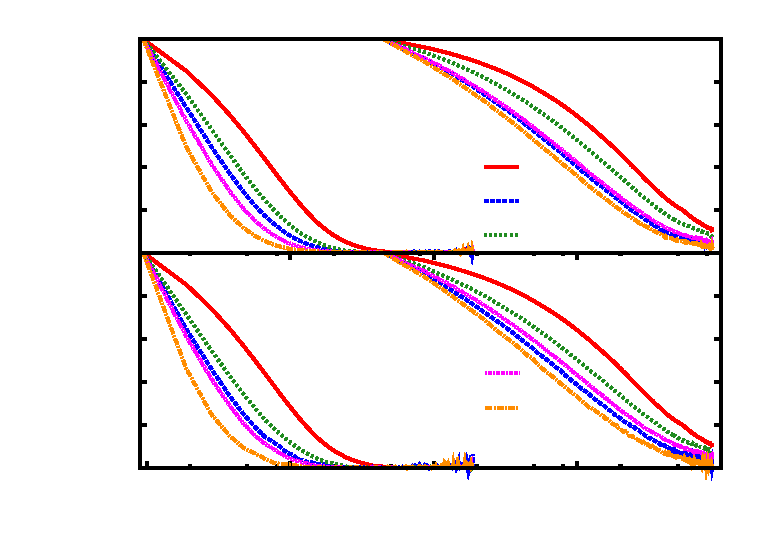
\includegraphics{./isf_qlm_normed}}%
    \gplfronttext
  \end{picture}%
\endgroup
